\documentclass{beamer}
%
% Choose how your presentation looks.
%
% For more themes, color themes and font themes, see:
% http://deic.uab.es/~iblanes/beamer_gallery/index_by_theme.html
%
\mode<presentation>
{
  \usetheme{default}      % or try Darmstadt, Madrid, Warsaw, ...
  \usecolortheme{default} % or try albatross, beaver, crane, ...
  \usefonttheme{default}  % or try serif, structurebold, ...
  \setbeamertemplate{navigation symbols}{}
  \setbeamertemplate{caption}[numbered]
} 

\usepackage[english]{babel}
\usepackage[utf8x]{inputenc}
\usepackage{amsmath}

\title[Your Short Title]{Bitcoin Allocation}
\author{Samuele Vianello}
%\institute{Where You're From}
\date{October 8th}

\begin{document}

\begin{frame}
  \titlepage
\end{frame}

% Uncomment these lines for an automatically generated outline.
\begin{frame}{Outline}
  \tableofcontents
\end{frame}

%\section{Introduction}

%\begin{frame}{Introduction}
%
%\begin{itemize}
%  \item Your introduction goes here!
%  \item Use \texttt{itemize} to organize your main points.
%\end{itemize}
%
%\vskip 1cm

%\begin{block}{Examples}
%Some examples of commonly used commands and features are included, to help you get started.
%\end{block}
%
%\end{frame}

\section{Models}

\subsection{Multivariate Merton}

\begin{frame}{Original Merton Model (1976)}
Original Merton 1976 model:
\begin{equation}
\label{merton_model}
    \frac{dS_t}{S_t} = \alpha dt + \sigma dW_t  + (Y_t-1)dN
\end{equation}

where 
\begin{itemize}
    \item $\alpha$ is the drift
    \item $\sigma$ is the diffusion coefficient
    \item $Y_t$ is a process modelling the intensity of the jumps
    \item $N(t)$ is the Poisson process driving the arrival of the jumps and has parameter $\lambda$
\end{itemize}

\end{frame}


\begin{frame}{Dynamics of the log-returns}
%%%%% add references to cont-tankov and martin
We can rewrite (\ref{merton_model}) in terms of the log-returns $X_t = log(S_t)$ and obtain:
\begin{equation}
    dX_t = (\alpha - \frac{\sigma^2}{2})dt + \sigma dW_t + \log (Y_t)
\end{equation}

that has as solution:
\begin{equation}
\label{merton_returns}
    X_t =X_0 +  \mu t + \sigma W_t + \sum_{k=1}^{N(t)} \eta_k
\end{equation}

where 
\begin{itemize}
    \item $X_0=log(S_0)$
    \item $\eta_k= \log(Y_k) = \log(Y_{t_k})$ and $t_k$ is the time when the $k^{th}$ Poisson shock from $N(t)$ happens
    \item $\mu = \alpha - \frac{\sigma^2}{2} $ for ease of notation
\end{itemize}

\end{frame}

\begin{frame}{Discretized dynamics of log-returns}

It is often useful when dealing with market data that are by nature discrete, to consider a \textit{discretized} version of (\ref{merton_returns}) in which the values are sampled at intervals of $\Delta t$ in $[0, T]$. We thus get that for $X_i = \log(\frac{S_{i+1}}{S_i})$:

\begin{equation}
\label{discrete_returns}
    X_i =  \mu \Delta t + \sigma \sqrt{\Delta t} \; z +  \sum_{k=1}^{N_{i+1} - N_i} Y_k
\end{equation}

where we denote $X_i = X_{t_i}$, $N_i = N(t_i)$ and $t_i = i \Delta t$ with $i= 0 \dots N$, $t_N = N \Delta t= T$,  $z$ is distributed as a standard Gaussian $ z\sim \mathcal{N}(0,1)$.

 Following basic stochastic analysis, one can prove that the resulting value $N_{i+1} - N_i$,  is distributed as a Poisson random variable $N$ of parameter $\lambda \Delta t$.
\end{frame}

\begin{frame}{Original Merton Model (1976)}
Applying the Total probability theorem, we get the following expression for the transition density:
\begin{equation}
\label{transitional}
    f_{\Delta X} (x) = \sum_{k=0}^{\infty} \mathbb{P}(N = k) f_{\Delta X | N = k}(x) 
\end{equation}

This infinite mixture of Gaussian random variable makes the MLE intractable(see Honore). %%% add reference 
To get a simpler definition of the log-return density, we limit our study to small values of $\lambda \Delta t$ so that the Poisson variable can only be in ${0,1}$ with non-negligible probability.
\begin{equation*}
\begin{split}
    f_{\Delta X} (x) & = \mathbb{P}(N = 0) f_{\Delta X | N = 0}(x) + \mathbb{P}(N = 1) f_{\Delta X | N = 1}(x)\\
             &= (1 - \lambda \Delta t) \;f_{\mathcal{N}}(x ; \mu, \sigma^2) + (\lambda \Delta t)\; f_{\mathcal{N}}(x ; \mu + \theta, \sigma^2+\delta^2)
\end{split}
\end{equation*}
\end{frame}

\begin{frame}{Multivariate Merton}
Multivariate generalization of Merton's 1976 \textit{jump diffusion} for $n$ assets:
\begin{equation}
\label{merton_prices}
    \frac{dS_t^{(j)}}{S_t^{(j)}} = \alpha_j dt + \sigma_j dW_t^{(j)} + (Y^{(j)}_t -1) dN^{(j)}_t
\end{equation}

where for $j = 1 ... n$ representing the assets:
\begin{itemize}
    \item $\mathbf{S}_t$ is the price vector
    \item $\alpha_j$ are the drifts
    \item $\sigma_j$ are the diffusion coefficients
    \item $W^{(j)}_t$ are the components of an $n$-dimensional Wiener process $ \mathbf{W}_t$ with $dW^{(j)}dW^{(i)}=\rho_{j,i}$
    \item $\eta_j$ represent the intensities of the jumps and are distributed as Gaussian: $\eta_j \sim \mathcal{N}(\theta_j , \delta_j^2)$
    \item $N^{(j)}(t)$ are Poisson processes with parameters $\lambda_j$, which are independent of $\mathbf{W}_t$ and of one another
\end{itemize}

\end{frame}


\begin{frame}{Multivariate transition density}
We can proceed as in the univariate case in order to get an explicit formula for the transition density, conditioning on all the different Poisson processes. In the two asset case we have
\begin{equation*}
\begin{aligned}
    f_{\Delta\mathbf{X}}(\mathbf{x}) &= \sum_{k_1=0}^{\infty}\sum_{k_2=0}^{\infty} \mathbb{P}(N^{(1)}(t) = k_1, N^{(2)}(t)=k_2) \\
    &f_{\Delta\mathbf{X}}(\mathbf{x} | N^{(1)}(t) = k_1, N^{(2)}(t)=k_2)\\
    &= \sum_{k_1=0}^{\infty}\sum_{k_2=0}^{\infty}\mathbb{P}(N^{(1)}(t) = k_1) \mathbb{P}(N^{(2)}(t)=k_2)\\
    &f_{\Delta\mathbf{X}}(\mathbf{x} | N^{(1)}(t) = k_1, N^{(2)}(t)=k_2)
\end{aligned}
\end{equation*}
Considering small $\Delta t$:
\begin{equation*}
\begin{aligned}
        f_{\Delta\mathbf{X}}(\mathbf{x}) = \sum_{k_1=0}^{1}\sum_{k_2=0}^{1} &\mathbb{P}(N^{(1)}(t) = k_1) \mathbb{P}(N^{(2)}(t)=k_2)\\ &f_{\Delta\mathbf{X}}(\mathbf{x}| N^{(1)}(t) = k_1, N^{(2)}(t)=k_2, N^{(Z)}(t)=k_Z )
\end{aligned}
\end{equation*}

\end{frame}

\begin{frame}{MLE procedure}
To recover the parameter of the model, we maximize the \textit{Likelihood} function:
    \begin{equation}
    \mathcal{L}(\psi | \Delta \mathbf{x}_{t_1},\Delta \mathbf{x}_{t_2},\dots,\Delta \mathbf{x}_{t_N}) = \sum_{i=1}^{N} f_{\Delta \mathbf{X}}(\Delta\mathbf{x}_{t_i} | \psi)
\end{equation}

We first use a stochastic optimization in which we find where the global minimun should be and then proceed with an algorithm that computes the numerical gradient to reach the closest minimum.

\end{frame}
\section{Calibration}
\subsection{Calibration Data}
\begin{frame}{Data}
\begin{itemize}
    \item Bitcoin
    \item 3 stock indices: S\&P500, Eurostoxx50 and MSCI BRIC
    \item 4 commodities: Gold, Oil, Industrial Metals and Grain
    \item 4 currencies  to USD: EUR, GBP, CHF and JPY
    \item 2 bond indices: BBG Barclays PAN EURO and PAN US Aggregate
\end{itemize}

Daily prices (working days only) from September 2010 to September 2018 provided by Bloomberg.

\end{frame}

\begin{frame}{Histogram of calibrated values}
\begin{figure}
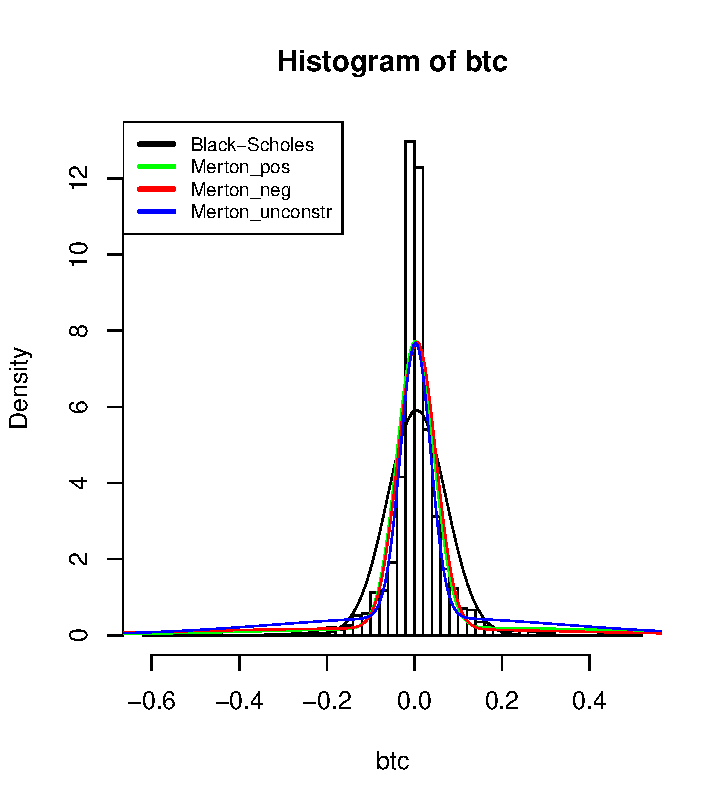
\includegraphics[width=0.8\textwidth]{historgram_10percent.pdf}
\label{roll_stocks}
\end{figure}
\end{frame}

\subsection{Calibration Results}
\begin{frame}{Parameter Results}
\begin{table}[]
\begin{tabular}{lllllllll}
     &btc	&bric	&sp500	&eurostoxx	&gold	&wti	&grain	\\
$\mu$ &1.5391	&0.0132	&0.1320	&0.0558	&0.0372	&0.0405	&-0.0444\\
$\theta$ &-0.10	&-0.10	&-0.10	&-0.10	&-0.10	&-0.10	&-0.10\\
$\delta$&0.1713	&0.0885	&0.1001	&0.0909	&0.0951	&0.1242	&0.1059 \\
$\lambda$&47.617	&0.976	&2.535	&1.364	&2.539	&9.459	&2.712	\\
\end{tabular}
\end{table}

\begin{table}[]
\begin{tabular}{lllllllll}
&metal	&eur	&gbp	&chf	&jpy	&pan-euro	&pan-us\\
$\mu$ &-0.0192	&-0.0148	&-0.0133	&0.0009	&-0.0143	&0.0410	&0.0259\\
$\theta$ &-0.10	&-0.10	&-0.10	&-0.10	&-0.10	&-0.10	&-0.10\\
$\delta$ &0.1029	&2.8356	&0.0987	&0.1150	&0.0933	&0.0912	&0.0998\\
$\lambda$ &0.793	&0.123	&0.898	&1.954	&1.593	&0.400	&0.641\\
\end{tabular}
\end{table} 
\end{frame}

\section{Correlation}
\begin{frame}{Correlation Significance}
\begin{table}[]
\begin{tabular}{lllllllll}
&bric	&sp500	&eurostoxx	&gold	&wti	&grain	&metal\\
Correlation &0.0115	&0.0398	&0.0364	&-0.0014	&0.0044	&0.0366	&0.0267\\
Pearson &0.577	&0.062	&0.091	&0.945	&0.835	&0.087	&0.214\\
Permutation &0.596	&0.066	&0.094	&0.950	&0.838	&0.092	&0.218\\
Spearman &0.666	&0.647	&0.188	&0.511	&0.945	&0.155	&0.821\\
\end{tabular}
\end{table} 

\begin{table}[]
\begin{tabular}{lllllllll}
&eur	&gbp	&chf	&jpy	&pan-euro	&pan-us\\
0.0267 &0.0233	&0.0071	&0.0235	&-0.0101	&-0.0247	&-0.0179\\
0.214 &0.286	&0.747	&0.267	&0.652	&0.242	&0.404\\
0.218 &0.283	&0.743	&0.279	&0.641	&0.254	&0.410\\
0.821 &0.411	&0.675	&0.990	&0.493	&0.429	&0.330\\
\end{tabular}
\end{table} 
\end{frame}


\begin{frame}{Rolling Correlation}
\begin{figure}
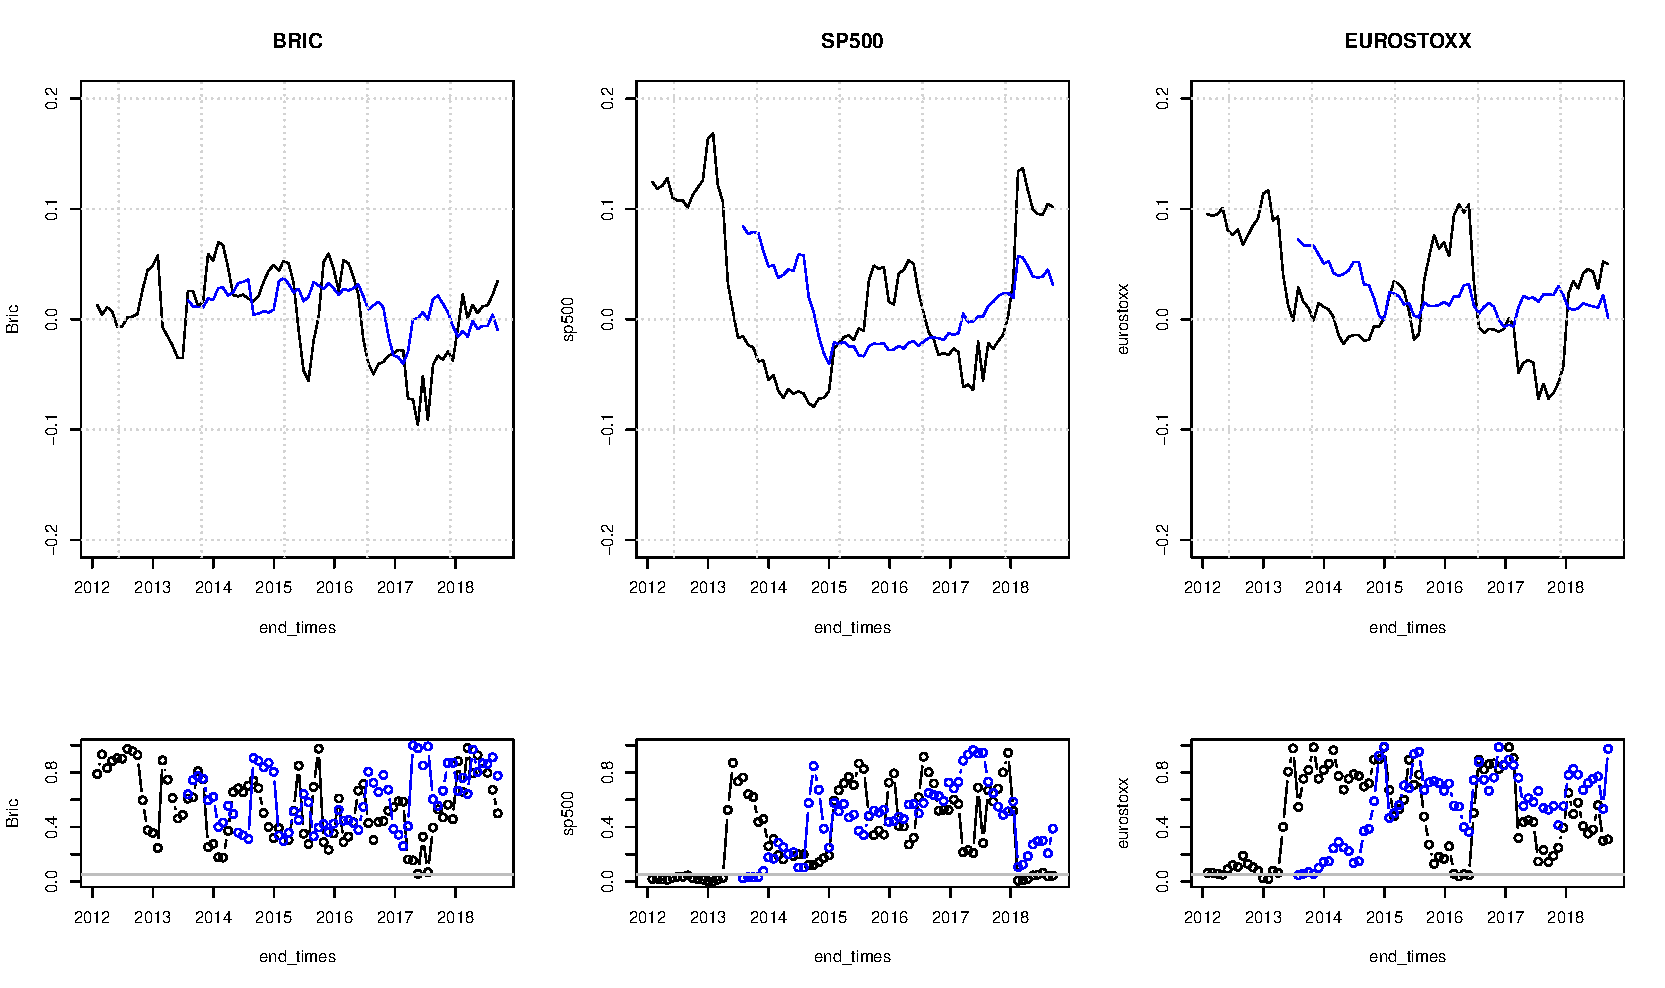
\includegraphics[width=\textwidth]{rolling_stocks.pdf}
\label{roll_stocks}
\end{figure}
\end{frame}

\begin{frame}{Rolling Correlation}
\begin{figure}
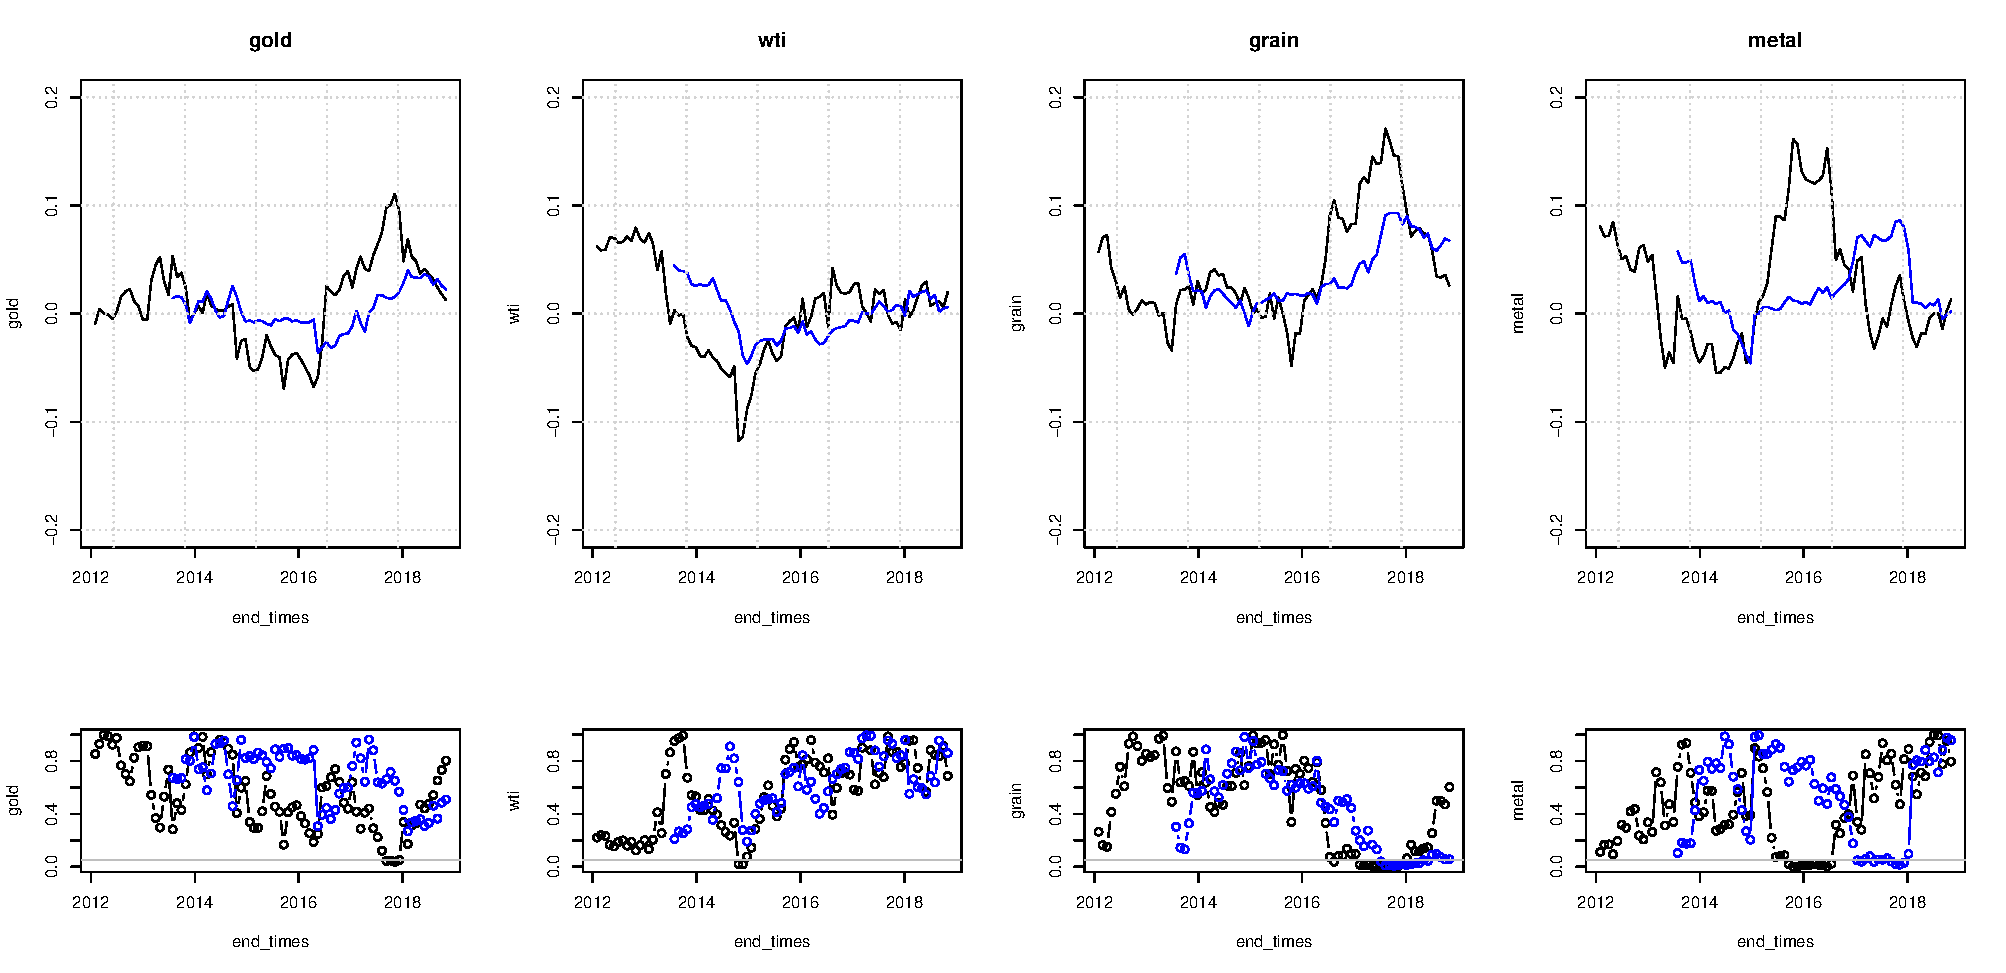
\includegraphics[width=\textwidth]{rolling_commodities.pdf}
\label{roll_stocks}
\end{figure}
\end{frame}

\begin{frame}{Rolling Correlation}
\begin{figure}
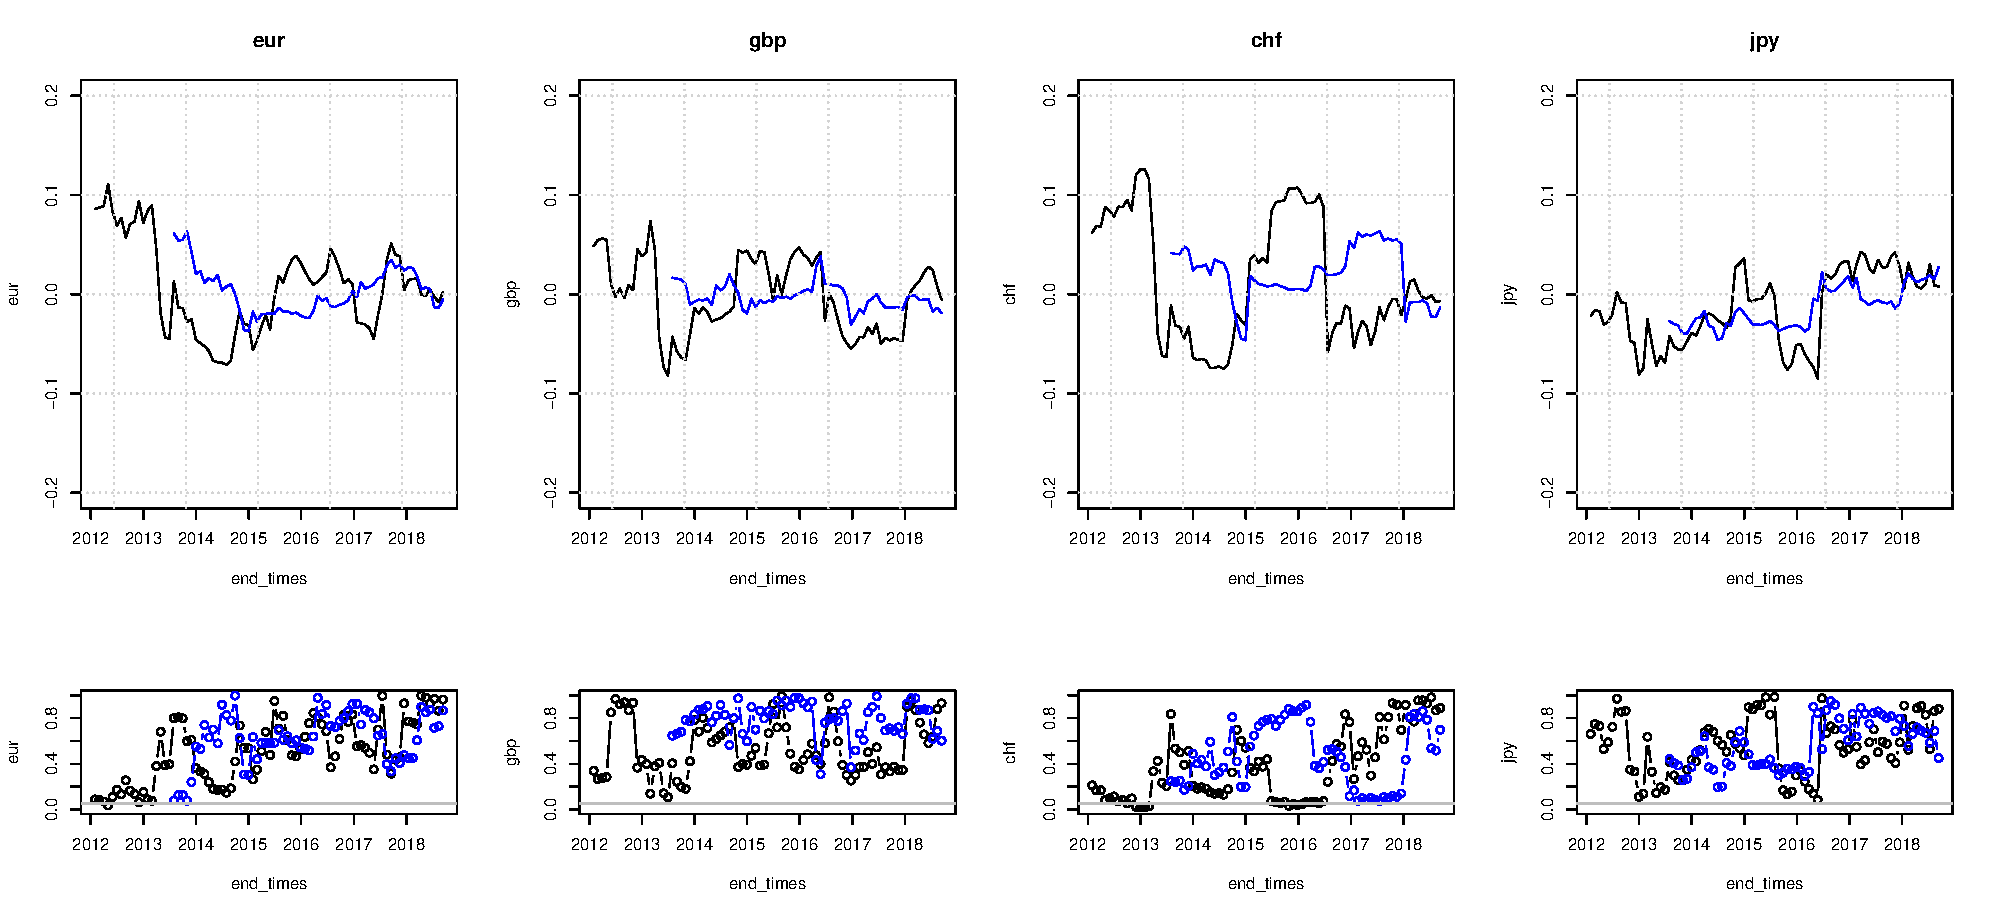
\includegraphics[width=\textwidth]{rolling_fx.pdf}
\label{roll_stocks}
\end{figure}
\end{frame}

\begin{frame}{Rolling Correlation}
\begin{figure}
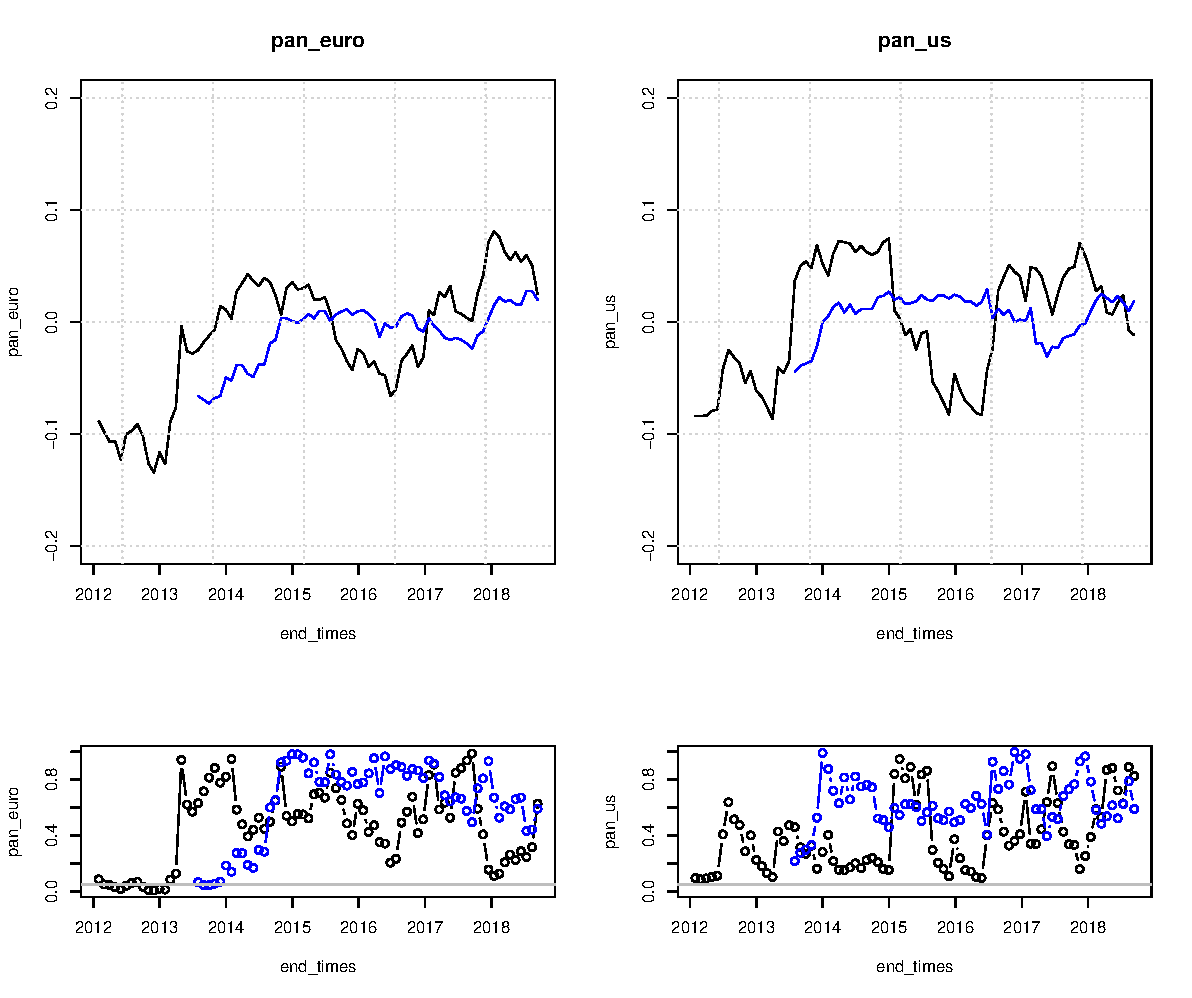
\includegraphics[width=0.8\textwidth]{rolling_bonds.pdf}
\label{roll_stocks}
\end{figure}
\end{frame}

\section{Efficient Frontier}

\begin{frame}{Efficient  Frontier and Optimal Allocation}
The two approaches consider both involve the minimization of a \textit{risk measure} given a level of target returns:
\begin{itemize}
	\item \textit{Markowitz Mean-Variance optimization}:  minimize the portfolio variance (or equivalently the volatility). This approach has explicit formulas for the solution in the unconstrained case.
	\item \textit{CVaR optimization}: minimize the portfolio \textit{conditional VaR} rather than the simple VaR due to the mathematical properties of the former (CVaR is a coherent risk measure). Numerical algorithms are required.
\end{itemize}
\end{frame}


\begin{frame}{Efficient  Frontier and Optimal Allocation}
General framework:
\begin{subequations}
	\begin{align}
	&\!\min_{\mathbf{w}\in \mathbb{R}^{n}}        & & PtfRisk(\mathbf{w}) \notag\\
	& \text{subject to} &      & \mathbf{e}'\mathbf{w} = 1 , \notag\\
	&                  &      & \mathbf{r}'\mathbf{w} = r_{target},\label{eq:constraint2} \notag\\
	&		 &        & w_{i} \geq 0, \text{for} \: i = 1\dots n. \notag
	\end{align}
\end{subequations}

where:
\begin{itemize}
	\item \textbf{w} is the vector of weights,
	\item \textbf{r} is the vector of returns,
	\item \textbf{e} indicates a vector of ones,
	\item $r_{target}$ is the target portfolio return.
\end{itemize}
\end{frame}

\begin{frame}{Markowitz Efficient Frontier}

****FIGURE OF UPDATED EFFICIENT FRONTIER********
%\begin{figure}
%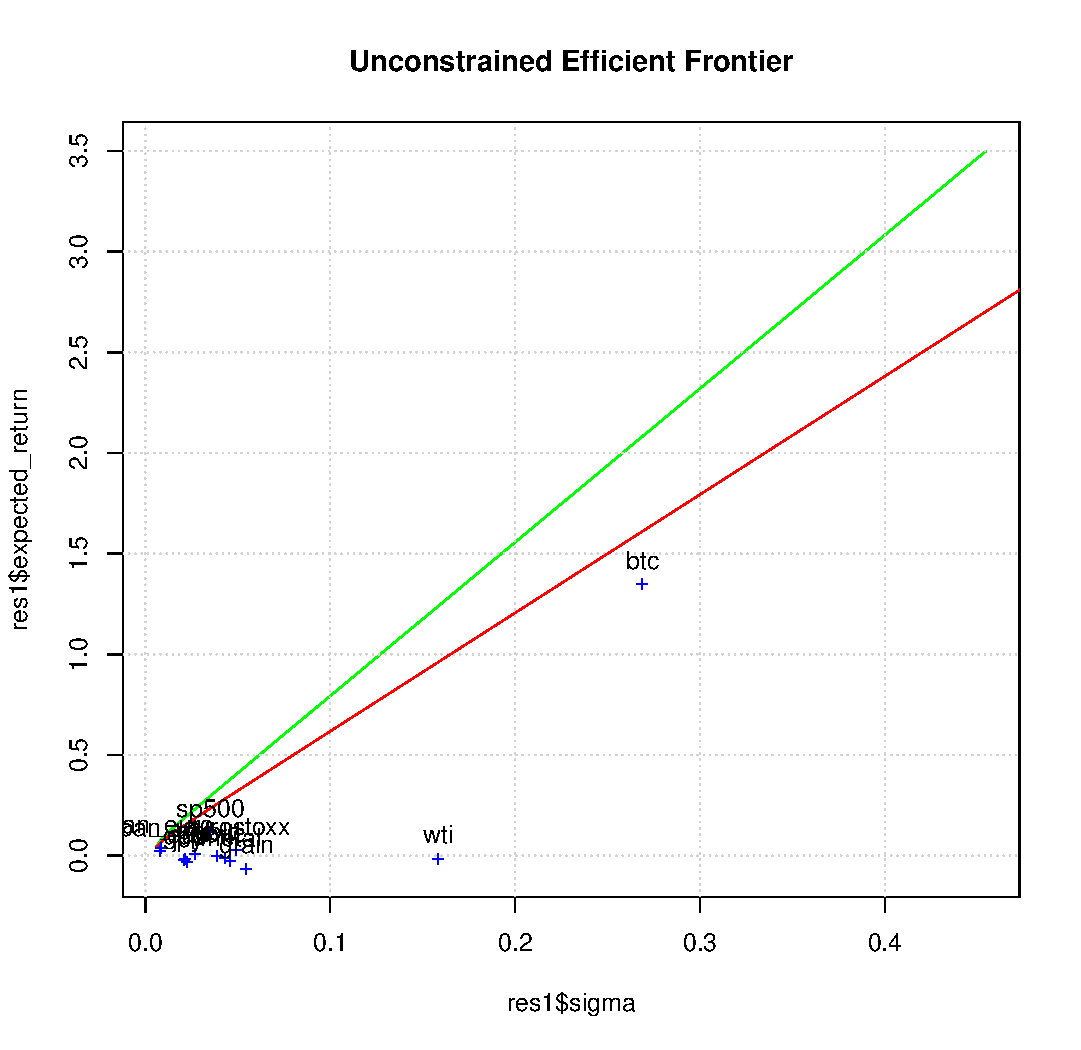
\includegraphics[width=0.8\textwidth]{unconstr_frontier.pdf}
%\label{roll_stocks}
%\end{figure}
\end{frame}

\begin{frame}{CVaR Efficient Frontier}
Since we only have the empirical distribution of the returns, we have to compute the CVaR empirically as well. We considered two approaches: 

\begin{enumerate}
	\item \textit{Annual returns simulation}: given the set of all available daily returns, extract 255 of them to simulate one annual return scenario. Repeat to get a number of simulations (in our case 10,000).
	We will refer to this method as annual bootstrap.
	\item \textit{Daily return as scenarios}: consider the latest $N = 255 * 5 = 1275$  daily return and use them as the different scenario realizations.
\end{enumerate}
\end{frame}

\begin{frame}{CVaR Efficient Frontier (annual bootstrap)}
***TWO FIGURES OF ANNUAL BOOTSTRAP FRONTIER****
\end{frame}

\begin{frame}{CVaR Efficient Frontier (daily returns)}
***********FIGURE OF DAILY RETURN FRONTIER**********
\end{frame}


\begin{frame}{Markowitz allocation}
\end{frame}


\end{document}
